\section{Cumplimiento de requerimientos}
El en la sección \ref{sec:req-ana} se expusieron los requerimientos funcionales y no funcionales para el sistema AutoSA. A continuación se exponen los cumplimientos de dichos requerimientos.

\subsection{Cumplimiento de requerimientos funcionales}
La sección \ref{sec:req-fun} lista los requerimientos funcionales del sistema AutoSA, de tales requerimientos se elaboraron los casos de uso, donde se describen los flujos que debe seguir el sistema AutoSA para cumplir con los requerimientos. Es así que a continuación se expone que la implementación del sistema satisface los requerimientos funcionales junto con los casos de uso y muestra la operación del usuario.

\subsubsection{Automatización de los procesos en el Sistema de Abastecimiento}
Los requerimientos funcionales \textbf{Automatización del proceso para contestar órdenes de reposición} y \textbf{Automatización del proceso para cotejar órdenes de reposición canceladas} automatizan los procesos descritos en la sección \ref{sec:desc-general} y son reflejados en los casos de uso \textbf{CU-CONTESTAAR} y \textbf{CU-VERIFICAR} (secciones \ref{cu-contestar} y \ref{cu-verificar}), la implementación es mostrada en la sección \ref{sec:agente}. El usuario puede ejecutar las automatizaciones desde la herramienta \textit{Sahi} de la siguiente forma:
\begin{itemize}
	\item Iniciar \textit{Sahi} sobre el explorar de Internet (punto 1 de la Figura \ref{fig:ss-sahi})
	\begin{figure}[h]
		\centering
		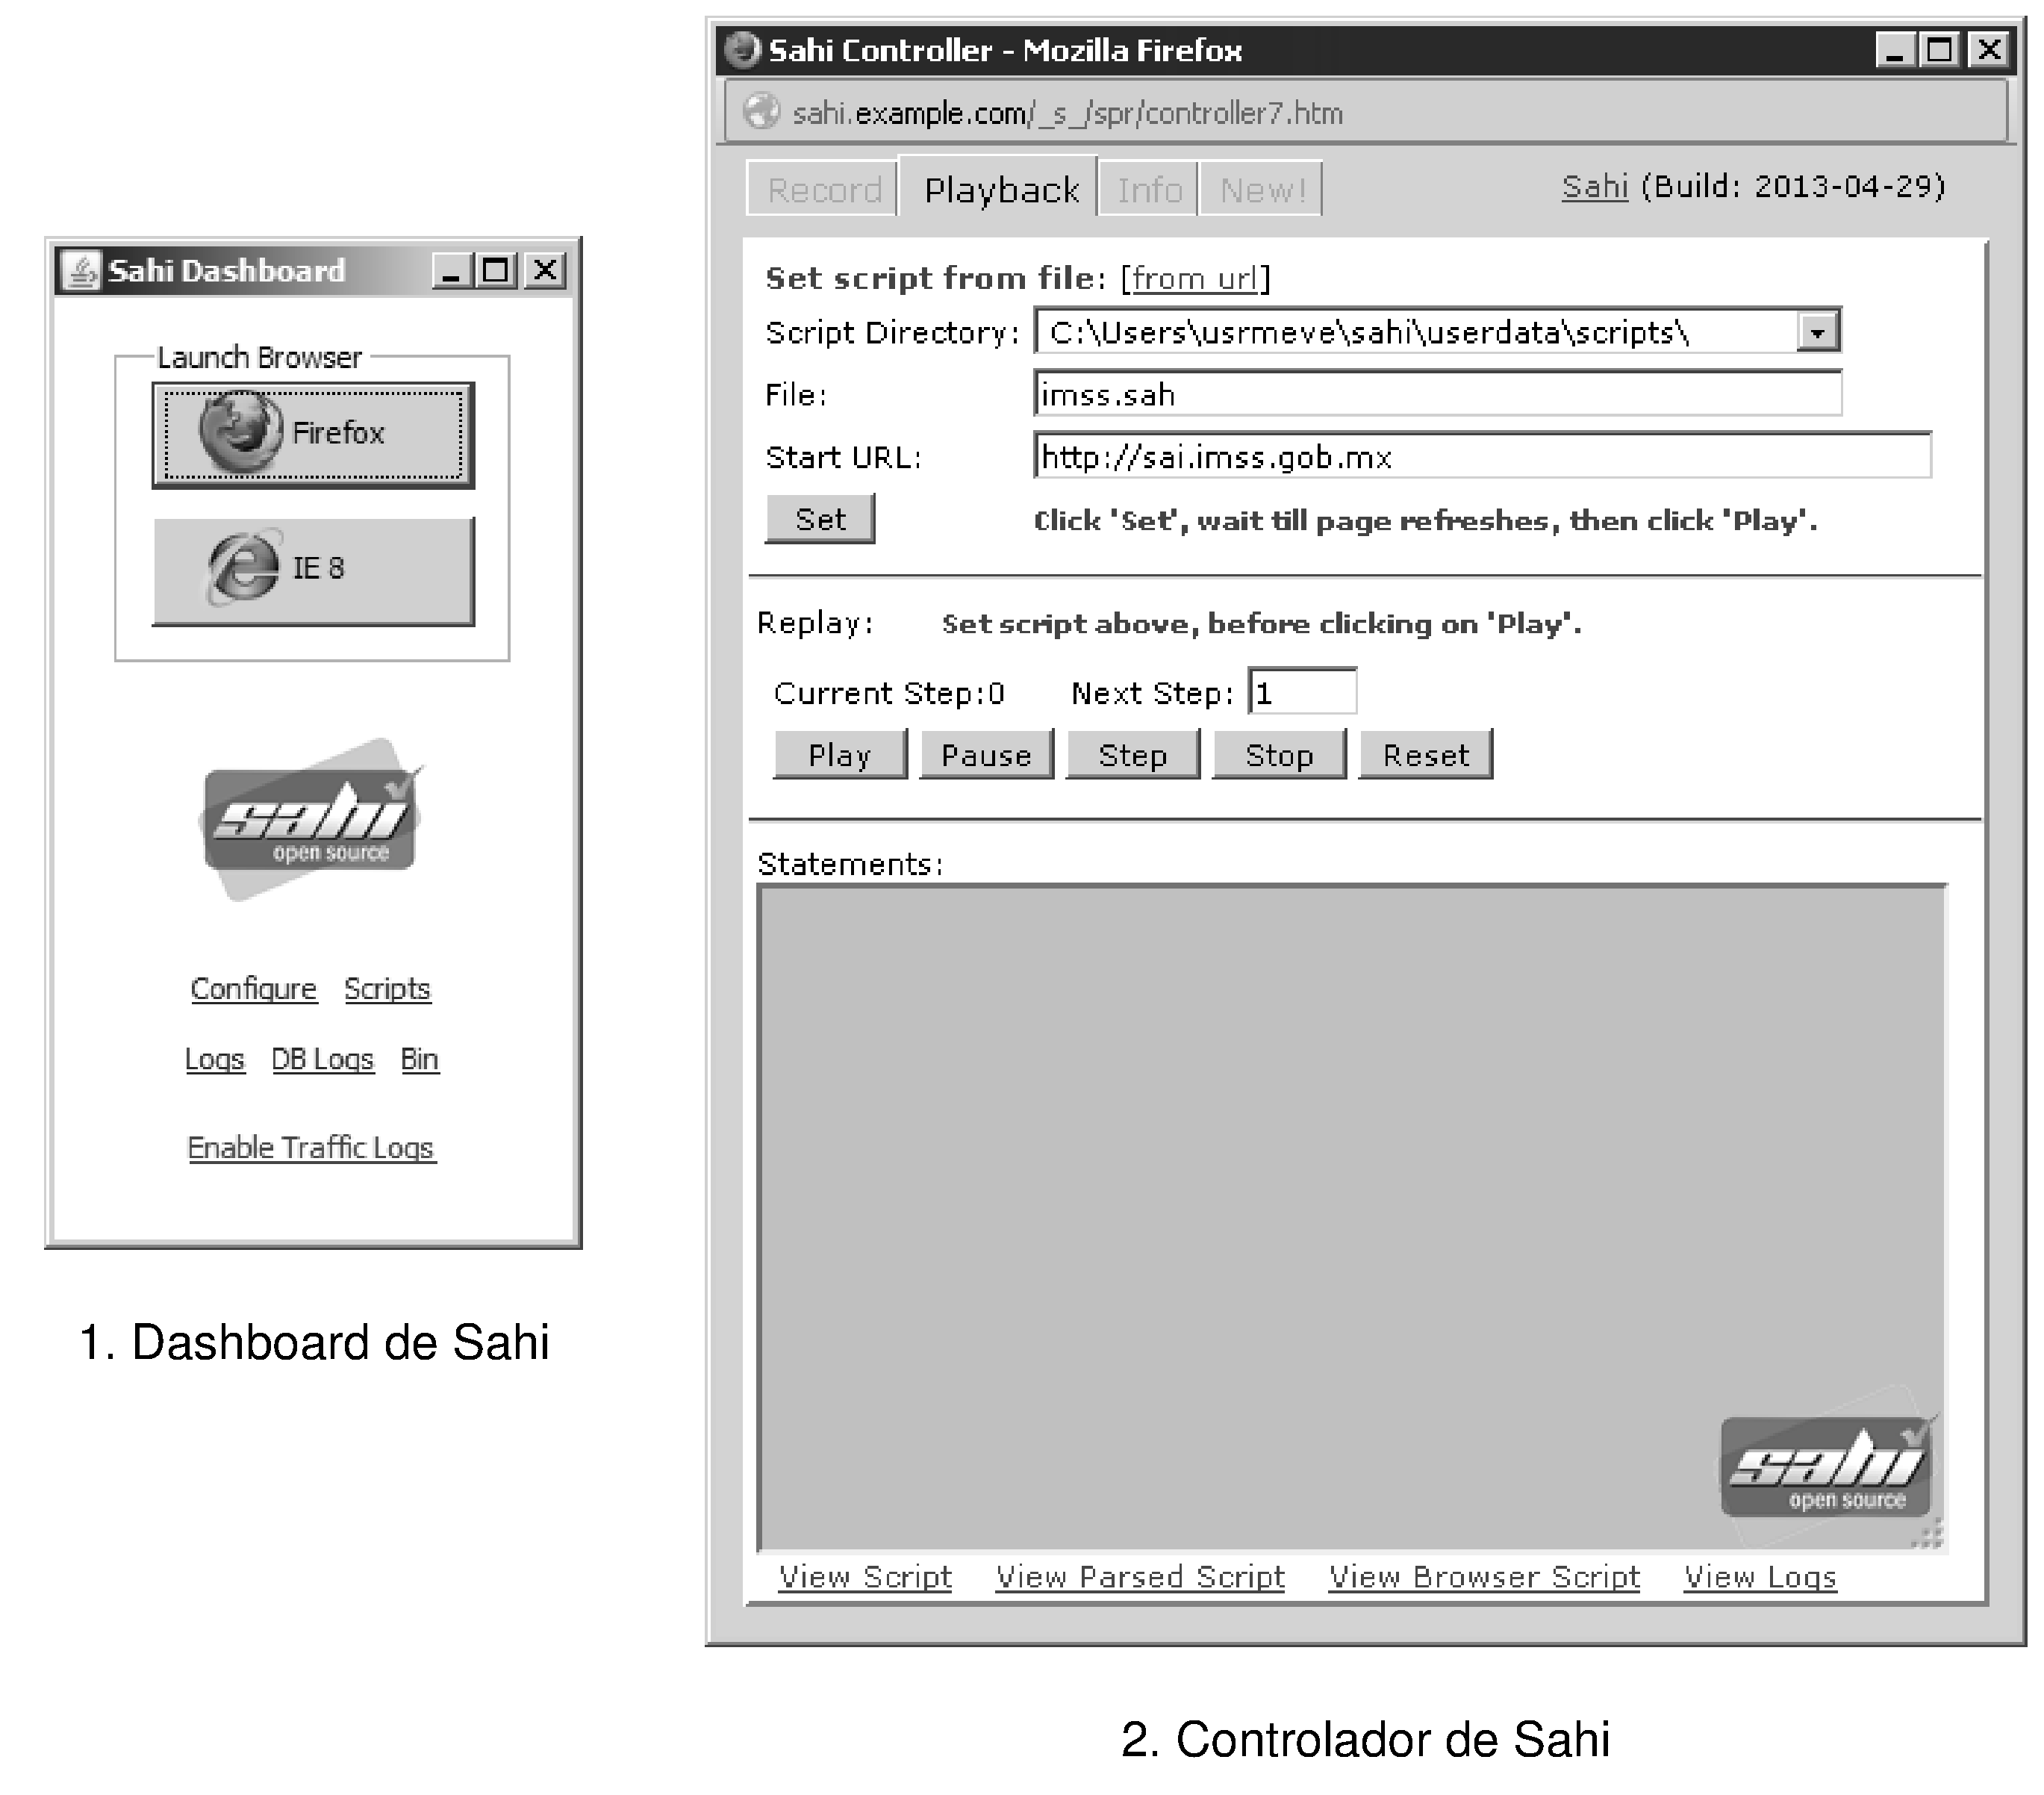
\includegraphics[scale=0.2]{ss-sahi}
		\caption{Interfaz de usuario de \textit{Sahi}.}
		\label{fig:ss-sahi}
	\end{figure}

	\item Iniciar el controlador de \textit{Sahi} y hacer los siguientes pasos (punto 2 de la Figura \ref{fig:ss-sahi}):
	\begin{enumerate}
		\item Seleccionar la rutina automatizada (contestar órdenes de reposición o verificación de órdenes de reposición).
		\item Ingresar la URL del \textit{Sistema de Abastecimiento}.
		\item Iniciar la ejecución.
	\end{enumerate}
\end{itemize}

%espaciado
\pagebreak
%espaciado

\subsubsection{Interfaz web para la administración de órdenes de reposición contestadas}
La interfaz web descrita en este requerimiento fue elaborada a lo largo de la sección \ref{sec:web-portal}, en particular los servicios de acceso y autorización fueron mostrados en el apartado 1 de la sección \ref{sec:backend}, asimismo, la pantalla de acceso fue descrita en el apartado 1 de la sección \ref{sec:frontend}.\\
Cabe mencionar que la pantalla de acceso es la primera pantalla que muestra la interfaz web (Figura \ref{fig:ss-login}).
\begin{figure}[h]
	\centering
	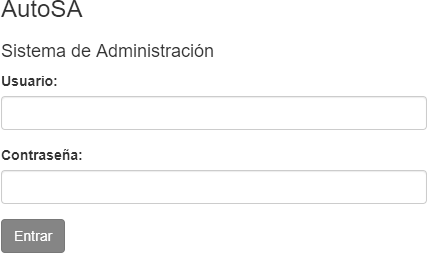
\includegraphics[scale=1.8]{ss-login}
	\caption{Pantalla de acceso a la interfaz web.}
	\label{fig:ss-login}
\end{figure}

\subsubsection{Búsqueda de órdenes de reposición}
La pantalla para la búsqueda de órdenes de reposición ofrece al usuario la posibilidad de buscar y visualizar órdenes de reposición, lo cual satisface al requerimiento \textbf{Búsqueda de órdenes de reposición}. La implementación de la pantalla y el comportamiento están descritos en el apartado 4 de la sección \ref{sec:frontend}. Por otra parte, la implementación de los servicios web que consume la pantalla de búsqueda de órdenes de reposición es mostrada en el apartado 2 de la sección \ref{sec:backend}.\\
El la Figura \ref{fig:ss-search} se observa la pantalla de búsqueda de órdenes de reposición.
\begin{figure}[h]
	\centering
	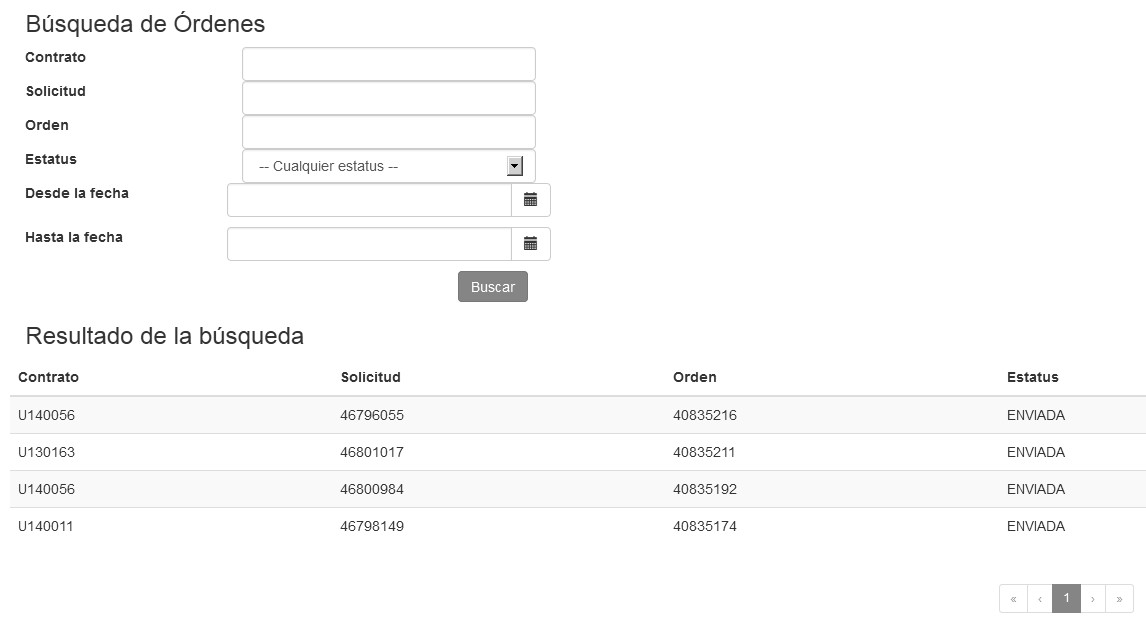
\includegraphics[scale=0.4]{ss-search}
	\caption{Pantalla de búsqueda de órdenes de reposición.}
	\label{fig:ss-search}
\end{figure}

\subsubsection{Visualización y edición de una orden de reposición}
Los requerimientos \textbf{Visualización de orden de reposición} y \textbf{Edición de órdenes de reposición} son plasmados en los casos de uso \textbf{CU-VISUALIZAR} y \textbf{CU-EDITAR} (secciones \ref{cu-visualizar} y \ref{cu-editar}). En la implementación y en la interfaz de usuario se utiliza la misma pantalla, como se muestra en la Figura \ref{fig:ss-edit}\footnote{Esta vista es descrita en el apartado 5 de la sección \ref{sec:frontend}. La implementación de los servicios web que consume la pantalla son mostrados en el apartado 2 de la sección \ref{sec:backend}.}.
\begin{figure}[h]
	\centering
	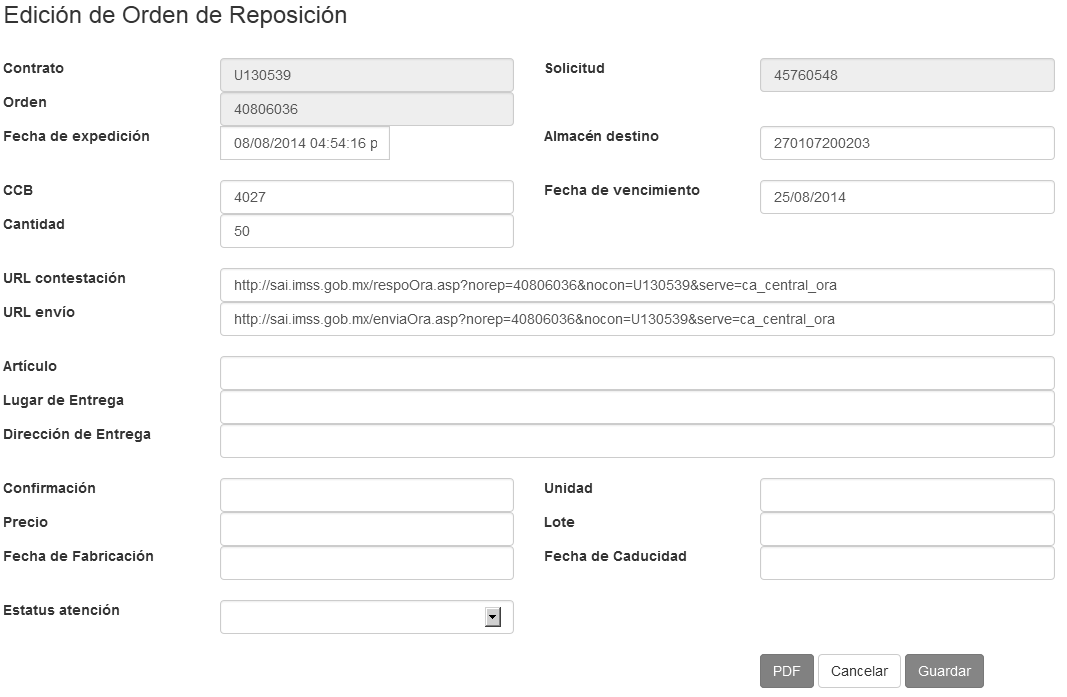
\includegraphics[scale=0.4]{ss-edit}
	\caption{Pantalla de búsqueda de órdenes de reposición.}
	\label{fig:ss-edit}
\end{figure}

\subsubsection{Generación de reportes}
La generación de reportes cumple con los requerimientos \textbf{Generación de reporte de órdenes de reposición contestadas}, \textbf{Generación de formato de salida} y \textbf{Generación de reporte con las órdenes de reposición canceladas recientemente}, mismos que son englobados en el caso de uso \textbf{CU-GENERAR-REPORTE} (sección \ref{cu-generar-reporte}). La implementación de la generación de reportes (sección \ref{sec:gen-repport}) y, a su vez, los servicios web que exponen esta funcionalidad están en el apartado 2 de la sección \ref{sec:backend}. La vista que ofrece al usuario la generación de reportes se encuentra en el apartado 2 de la sección \ref{sec:frontend}, en la Figura \ref{fig:ss-report} se observa la pantalla para la generación de reportes\footnote{Por acuerdo de confidencialidad no se puede mostrar el contenido de los reportes generados.}. 
	\begin{figure}[h]
		\centering
		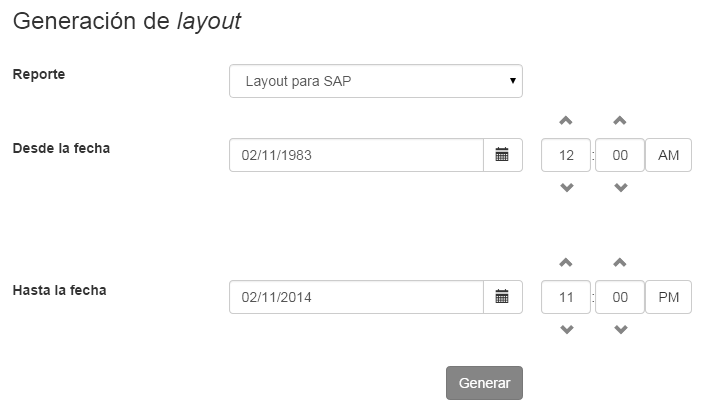
\includegraphics[scale=0.5]{ss-report}
		\caption{Pantalla de generación de reportes.}
		\label{fig:ss-report}
	\end{figure}

\subsubsection{Actualización de catálogos y estatus de órdenes de reposición canceladas}
Los requerimientos \textbf{Actualización de catálogos} y \textbf{Actualización de estatus de órdenes de reposición canceladas} son modelados en el caso de eso \textbf{CU-ACTUALIZAR-CATALOGO}, la implementación de la actualización a los datos es dada en la sección \ref{sec:persistence-web}, y la implementación del servicio web se encuentra en el apartado 2 de la sección \ref{sec:backend}. La implementación de la vista está dada en el apartado 3 de la sección \ref{sec:frontend}, en la Figura \ref{fig:ss-catalog} muestra pantalla de la administración de catálogos\footnote{Por acuerdo de confidencialidad no se puede mostrar el contenido de los catálogos.}.
\begin{figure}[h]
	\centering
	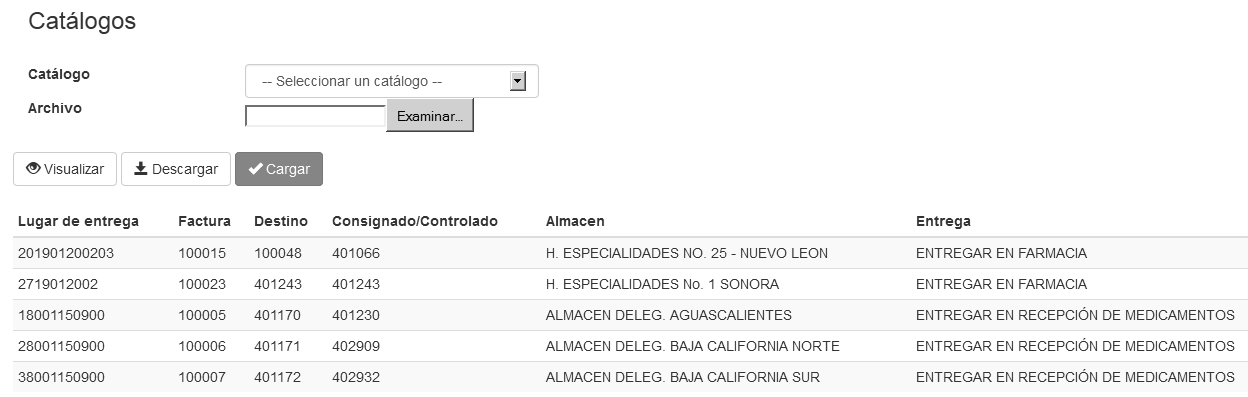
\includegraphics[scale=0.4]{ss-catalog}
	\caption{Pantalla de administración de catálogos.}
	\label{fig:ss-catalog}
\end{figure}


\subsection{Cumplimiento de requerimientos no funcionales}
En la sección \ref{sec:nonfunctional-req} se enlistan los requerimientos no funcionales para el sistema AutoSA.

\subsubsection{Ejecución del Sistema AutoSA en los sistemas operativos más comunes.}
En la sección \ref{sec:java} se menciona que el lenguaje de programación \textit{Java} es multiplataforma gracias a que el código escrito por los desarrolladores es traducido a \textit{Bytecode} y es este último el que ejecuta la Máquina Virtual de \textit{Java}. Existen implementaciones de robustas y ampliamente probadas de la Máquina Virtual de \textit{Java} para una gran variedad de sistemas operativos. Es por esta razón que se decidió utilizar a \textit{Java} como el lenguaje de programación principal.

\subsubsection{Base de datos relacional SQL}
Al principio del proyecto, la farmacéutica sentó que de ser necesaria una base de datos, el área encargada de las bases de datos de la farmacéutica sería quien proveería tanto la infraestructura y como la base de datos relacional, por lo que las rutinas DDL y DML (sección \ref{sec:impl-db}) y las consultas del módulo de persistencia (sección \ref{sec:persistence}) siguen los estándares SQL mostrados en la sección \ref{sec:bd-r}.

